\documentclass[12pt,a4paper,oneside]{article}
% Nastavení znakové sady Unicode
\usepackage{cmap}
\usepackage[a4paper,left=35mm,right=30mm,top=30mm,bottom=30mm]{geometry}
\usepackage[czech]{babel}
\usepackage[utf8]{inputenc}
\usepackage[T1]{fontenc}
\usepackage[dvipsnames]{xcolor}
\usepackage{float}
\usepackage{graphicx}
\usepackage{hyperref}
\usepackage{index}
\usepackage{listings}
\usepackage{url}
\usepackage{enumitem}
\newcommand\YAMLcolonstyle{\color{red}\mdseries}
\newcommand\YAMLkeystyle{\color{black}\bfseries}
\newcommand\YAMLvaluestyle{\color{blue}\mdseries}

\makeatletter

% here is a macro expanding to the name of the language
% (handy if you decide to change it further down the road)
\newcommand\language@yaml{yaml}

\expandafter\expandafter\expandafter\lstdefinelanguage
\expandafter{\language@yaml}
{
  keywords={true,false,null,y,n},
  keywordstyle=\color{darkgray}\bfseries,
  basicstyle=\YAMLkeystyle,                                 % assuming a key comes first
  sensitive=false,
  comment=[l]{\#},
  morecomment=[s]{/*}{*/},
  commentstyle=\color{purple}\ttfamily,
  stringstyle=\YAMLvaluestyle\ttfamily,
  moredelim=[l][\color{orange}]{\&},
  moredelim=[l][\color{magenta}]{*},
  moredelim=**[il][\YAMLcolonstyle{:}\YAMLvaluestyle]{:},   % switch to value style at :
  morestring=[b]',
  morestring=[b]",
  literate =    {---}{{\ProcessThreeDashes}}3
                {>}{{\textcolor{red}\textgreater}}1     
                {|}{{\textcolor{red}\textbar}}1 
                {\ -\ }{{\mdseries\ -\ }}3,
}

% switch to key style at EOL
\lst@AddToHook{EveryLine}{\ifx\lst@language\language@yaml\YAMLkeystyle\fi}
\makeatother

\newcommand\ProcessThreeDashes{\llap{\color{cyan}\mdseries-{-}-}}

\setlist{nolistsep}
\author{Roman Ondráček}
\title{Dálkové ovládání domácích spotřebičů mobilním telefonem}
% Vytvoření seznamu použitých zkratek
\newindex{zkr}{zdx}{znd}{Seznam použitých zkratek}
\lstset{
  inputencoding=utf8
}
\begin{document}
% Řádkování 1,5
\renewcommand{\baselinestretch}{1.5}
% Vynechání číslování
\pagestyle{empty}
\begin{center}
\large \textbf{STŘEDOŠKOLSKÁ ODBORNÁ ČINNOST} \\

\vspace{48mm}
% Český název
\huge \textbf{Dálkové ovládání domácích spotřebičů mobilním telefonem} \\

\vspace{64mm}
\end{center}

\begin{tabbing}
% Nastavení zarážek
\hspace{4mm} \= \hspace{24mm} \= \kill
\> \large \textbf{Autor:}  \> \large{Roman Ondráček}                                    \\[4mm]
\> \large \textbf{Škola:}  \> \large{Gymnázium Boskovice, příspěvková organizace}       \\[4mm]
\> \large \textbf{Kraj:}   \> \large{Jihomoravský}                                      \\[4mm]
\> \large \textbf{Obor:}   \> \large{10. Elektrotechnika, elektronika a telekomunikace} \\[24mm]
\> \large \textbf{Boskovice 2017}
\end{tabbing}

\newpage
% Zakázání číslování
\pagestyle{empty}
\begin{center}
\large \textbf{STŘEDOŠKOLSKÁ ODBORNÁ ČINNOST} \\

\vspace{48mm}
% Český název
\huge \textbf{Dálkové ovládání domácích spotřebičů mobilním telefonem} \\
\vspace{24mm}
% Anglický název
\huge \textbf{The remote control of home appliances via a mobile phone} \\

\vspace{24mm}
\end{center}

\begin{tabbing}
% Nastavení zarážek
\hspace{4mm} \= \hspace{24mm} \= \kill
\> \large \textbf{Autor:}     \> \large{Roman Ondráček}                                    \\[4mm]
\> \large \textbf{Škola:}     \> \large{Gymnázium Boskovice, příspěvková organizace}       \\[4mm]
\> \large \textbf{Kraj:}      \> \large{Jihomoravský}                                      \\[4mm]
\> \large \textbf{Školitel:}  \> \large{prof. Ing. Václav Říčný, CSc.}                     \\[4mm]
\> \large \textbf{Obor:}      \> \large{10. Elektrotechnika, elektronika a telekomunikace} \\[16mm]
\> \large \textbf{Boskovice 2017}
\end{tabbing}

\normalsize

\newpage

~ \vspace{128mm}

\section*{Prohlášení}

Prohlašuji, že svou práci na téma Dálkové ovládání domácích spotřebičů mobilním telefonem jsem vypracoval samostatně pod vedením prof. Ing. Václava Říčného, CSc. a s~použitím odborné literatury a dalších informačních zdrojů, které jsou všechny citovány v~práci a uvedeny v~seznamu literatury na konci práce. \\
Dále prohlašuji, že tištěná i elektronická verze práce SOČ jsou shodné a nemám závažný důvod proti zpřístupňování této práce v~souladu se zákonem č.~121/2000 Sb., o~právu autorském, o~právech souvisejících s~právem autorským a změně některých zákonů (autorský zákon) v~platném změní. \\[8mm]
V~Boskovicích dne \today \hspace{24mm} Podpis:

\newpage

~ \vspace{110mm}

\section*{Poděkování}

Děkuji svému školiteli prof. Ing. Václavu Říčnému CSc. za obětavou pomoc a podnětné připomínky, které mi během práce poskytoval. \\
Tato práce byla provedena za finanční podpory Jihomoravského kraje.

\vspace{8mm}
% Loga
\begin{figure}[!htb]
\minipage{0.50\textwidth}
	
\includegraphics[width = 64mm]{img/logo/jmk.pdf} \\[8mm]
	
\includegraphics[width = 64mm]{img/logo/jcmm.jpg}
\endminipage
\minipage{0.50\textwidth}
	
\includegraphics[width = 64mm]{img/logo/vut.pdf}
\endminipage
\end{figure}

\newpage

\section*{Anotace}

Cílem této práce je navrhnout a sestavit chytrou zásuvku, která se ovládá pomocí pomocí SMS a která může spínat odporovou zátěž až 10~A. Součástí mé práce je technická dokumentace výrobku, popis postupu výroby a samotný výrobek.

\subsection*{Klíčová slova}

GSM; SMS; IQRF; relé

\section*{Annotation}

The goal of this work is to design and build a smart power socket, which is controlled by a text message and which can switch resistive loads up to current 10~A. My work includes technical documentation, a description of the manufacturing process and the product itself.

\subsection*{Keywords}

GSM; text message; IQRF; relay

\newpage

% Nastavení číslování od Obsahu
\setcounter{page}{1}

\tableofcontents

\newpage

% Povolení číslování
\pagestyle{plain}

\section*{Úvod}

\addcontentsline{toc}{section}{Úvod}

V~posledních létech je ve středu pozornosti tzv. Internet věcí (IoT\index[zkr]{IoT!Internet of things|textit}) a chytrá domácnost. Na trhu jsou nabízeny chytré zásuvky, které však obvykle ovládány na kratší vzdálenosti a nenabízejí možnost pohodlně a bezpečně je ovládat vzdáleně pomocí mobilního telefonu. \\

Obvykle jsou tyto chytré zásuvky ovládány pomocí komunikace WiFi, která používá kmitočtové pásmo 2,4 GHz. Tato frekvence je hlavně ve městech hodně zarušená, protože se používá i pro přenosy jiných dat\cite{wiki/ism-band}. A proto většinou tyto chytré zásuvky lze ovládat pouze v~místní síti (LAN\index[zkr]{LAN!Local area network|textit}). Tento projekt má tedy umožnit ovládat tyto zásuvky (a tedy i elektrické spotřebiče v~nich zapojené) z~libovolné vzdálenosti. Navržený systém dálkového ovládání pomocí mobilního telefonu by měl, kromě vlastního ovládání, zabezpečit i přenos informace uživateli o~aktuálním stavu zásuvky. Cílem projektu je tedy návrh takové dálkově ovládané chytré zásuvky, její realizace a ověření funkčního vzorku. \\

Většina chytrých zásuvek obsahuje pouze jedno relé\cite{teardown-wemo-switch}, protože musí se povinně spínat fáze (spínání nulového vodiče je nepovinné). To přináší problém, protože například ve Francii, kde se stejně jako v~České republice použita zásuvka typu E\cite{zasuvka-typ-e}, je zdířka fáze umístěna vpravo nikoliv vlevo jako v~České republice\cite{faze-vlevo-nebo-vpravo}. Proto navržené řešení obsahuje i druhé relé pro spínání nulového vodiče. \\

Pro řešení zadání projektu jsem se rozhodl použít technologii IQRF. Je to technologie vyvinutá českou firmou Microrisc s.r.o., která se poměrně často používá ve světě internetu věcí a jiných systémů pro bezdrátový přenos malých objemů dat. Firma dává k~dispozici relativně malé moduly, které je možno integrovat do konkrétních zákaznických řešení.

\newpage

\section{Návrh hardware}

\subsection{Chytrá zásuvka}

Chytrá zásuvka je napájena ze sítě pomocí modulového spínaného zdroje do desky plošných spojů MEAN WELL IRM-02-5, který má výstupní napětí 5~V a maximální výstupní proud je 400~mA. \\

Chytrá zásuvka je řízena bezdrátovým modulem IQRF DCTR-72DAT, který spíná SMD\index[zkr]{SMD!Surface-mounted device|textit} unipolární tranzistory N-MOSFET\index[zkr]{N-MOSFET!N-Channel metal–oxide–semiconductor field-effect transistor|textit} BSS138. Ty spínají které spínají cívky dvou relé (jedno je použito pro spínání fáze a druhé relé je použito pro spínání nulového vodiče) OMRON G5Q-1A4-EU. \\

Při rozepnutí proudu v~cívce relé vzniká vlivem její indukčnosti napěťová špička, která může zničit spínací tranzistor. Proražení tranzistoru lze zabránit diodou paralelně zapojenou k~relé, která při rozepnutí relé uzavře obvod kolem indukčnosti. Použil jsem usměrňovací diodu 1N4007. Abych zabránil jiskření na kontaktech relé, jsem použil varistor MOV\index[zkr]{MOV!Metal Oxide Varistor|textit} SR PASSIVES VAR10-250.

\newpage

\subsubsection{Bezdrátový modul IQRF DCTR-72DAT}

V~chytré zásuvce jsem použil bezdrátový modul IQRF DCTR-72DAT, který rovněž vyrábí česká firma MICRORISC s.r.o., která sídlí v~Jičíně. Plošný spoj modulu má podobné rozměry jako SIM\index[zkr]{SIM!Subscriber identity module|textit} karta, proto je pro jeho připojení s~deskou plošných spojů použit konektor pro SIM karty. \\

\begin{figure}[H]
\centering
\label{fig:iqrf/fotka}
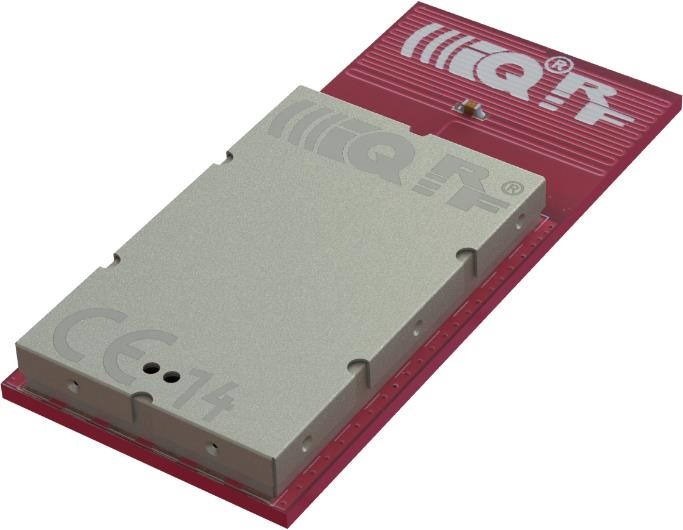
\includegraphics[width = 64mm]{img/iqrf/dctr-72dat.png}
\caption{Fotografie bezdrátového modulu}
\end{figure}

Modul může vysílat na bezlicenčních pásmech 916~MHz, která je určené pro Ameriku, a 868~MHz, určené pro zbytek světa. Vysílací výkon modulu je 12,5~mW, používá GFSK\index[zkr]{GFSK!Gaussian frequency-shift keying|textit} modulaci. Modul má integrovanou anténu na svém plošném spoji. \\

Pro komunikaci používá tzv. mesh neboli smíšenou topologii. Ta má výhody v~robustnosti a v~absenci centrálního prvku. Její nevýhodou je naopak potřebná ochrana proti zacyklení a nutnost směrování provozu. \\

Modul lze napájet napětím 3,1~V až 5,5~V, protože obsahuje LDO\index[zkr]{LDO!Low-dropout|textit} napěťový stabilizátor Microchip MCP1700T-3002E/TT. Dále modul obsahuje mikrokontrolér Microchip PIC16LF1938. Ten užívá operační systém IQRF OS, který za uživatele zajišťuje komunikaci s~integrovaným obvodem STMicroelectronics Spirit1. Tento obvod řídí bezdrátový datový přenos a má hardwarovou podporu blokové šifry AES-128\index[zkr]{AES!Advanced Encryption Standard|textit}. Operační systém dále ovládá integrované periferie (například digitální teploměr). IQRF DPA\index[zkr]{DPA!Direct Peripheral Access|textit} a uživatelská aplikace. Dále modul obsahuje digitální teploměr Microchip MCP9808E/MC. \\

Microchip PIC16LF1938 je 8-bitový mikrokontrolér s~architekturou PIC, která používá architekturu RISC\index[zkr]{RISC!Reduced instruction set computing|textit}, jenž má omezenou instruktážní sadu a rychlé vykonávání instrukcí. Flash paměť pro program má velikost 28~kB, paměť EEPROM má velikost 256~B a paměť SRAM má velikost 1~kB.

\begin{figure}[H]
\centering
\label{fig:iqrf/zjednodusene-schema}
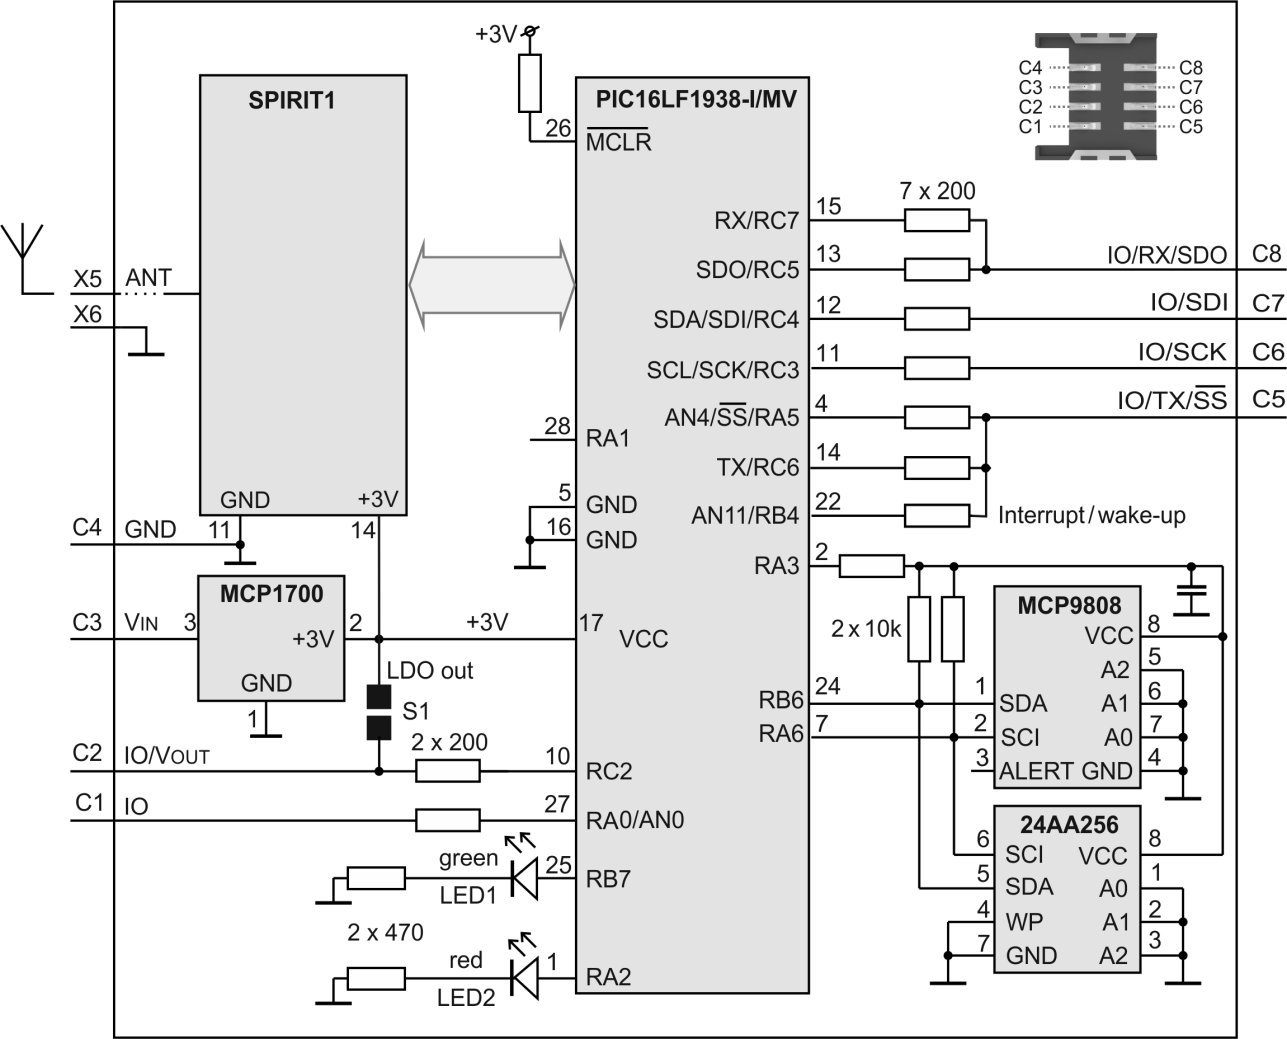
\includegraphics[width = 128mm]{img/iqrf/dctr-72dat-zjednodusene-schema.png}
\caption{Zjednodušené schéma bezdrátového modulu}
\end{figure}

Přestože je v~integrovaném obvodu řídící radiovou komunikaci hardwarová podpora šifry AES-128, tak podpora této šifry není v~IQRF OS\index[zkr]{OS!Operating system|textit}\index[zkr]{OS!Operační systém|textit} ještě implementována a místo ní se používá upravená bloková šifra XTEA\index[zkr]{XTEA!eXtended Tiny Encryption Algorithm|textit}, která je však méně bezpečná. Bloková šifra AES-128 bude implementovaná v~IQRF OS ve verzi 4.0, která má vyjít v~prvním čtvrtletí roku 2017.

\newpage

\subsubsection{Blokové schéma}

Na obrázku č.~3 se nachází blokové schéma chytré zásuvky, které popisuje její zapojení. Obrázek byl vytvořený v~open-source programu Dia\cite{sw/dia}.

\begin{figure}[H]
\centering
\label{fig:blokove-schema-zasuvky}
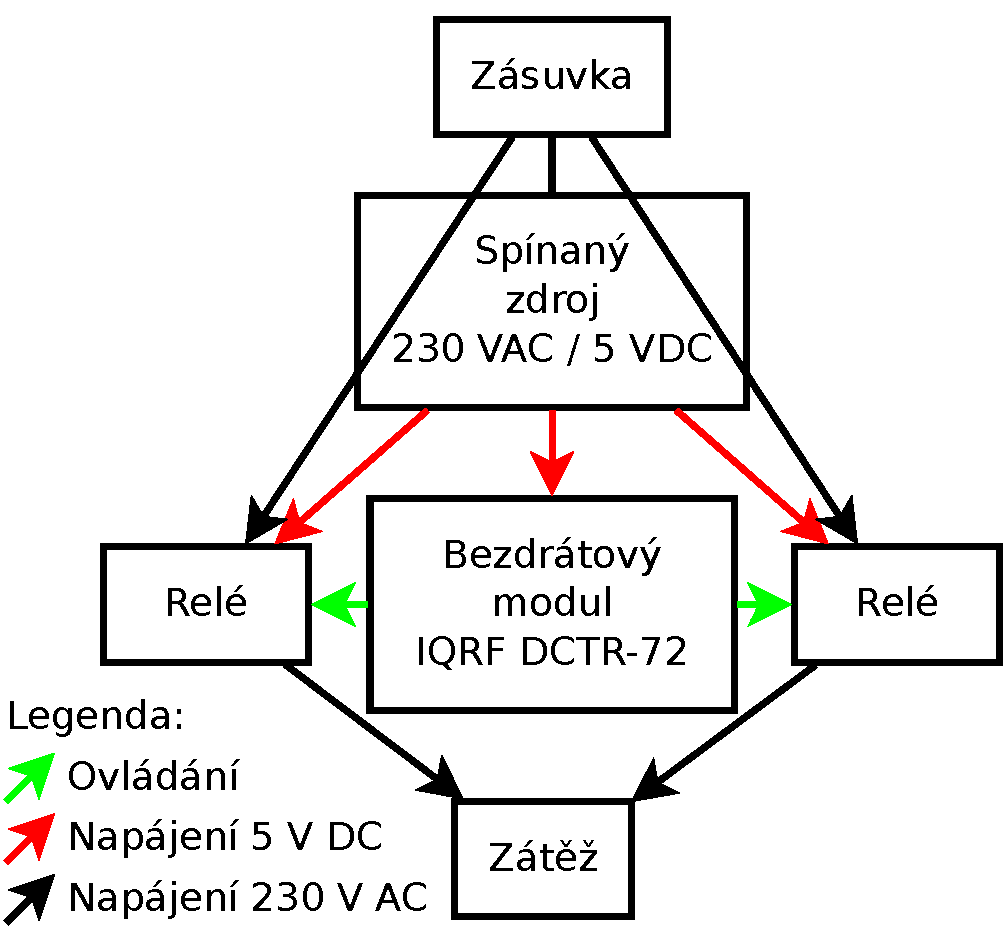
\includegraphics[width = 128mm]{img/blokove-schema/zasuvka.pdf}
\caption{Blokové schéma chytré zásuvky}
\end{figure}

\newpage

\subsubsection{Obvodové schéma}

Na obrázku č.~4 se nachází obvodové schéma chytré zásuvky. Obrázek je vytvořen v~open-source programu KiCad\cite{sw/kicad}.

\begin{figure}[H]
\centering
\label{fig:schematic}
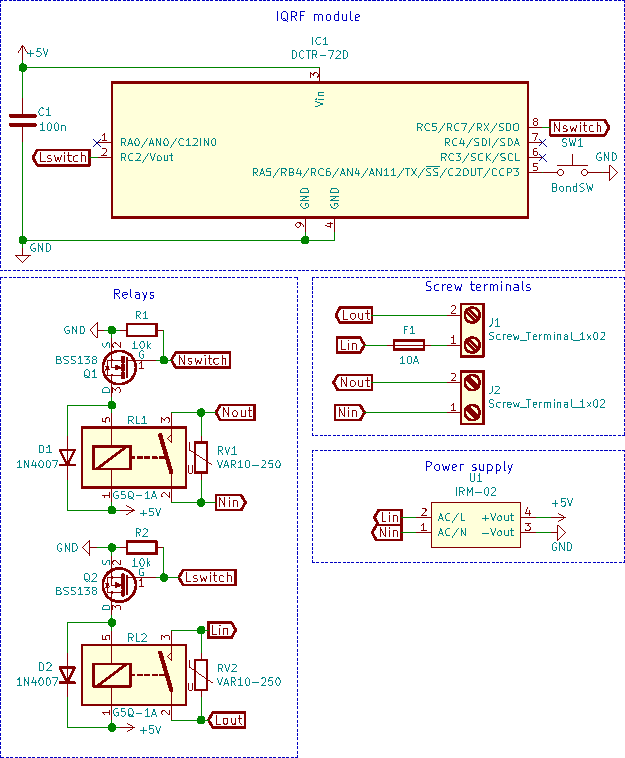
\includegraphics[width = 128mm]{img/kicad/schematic.pdf}
\caption{Obvodové schéma chytré zásuvky}
\end{figure}

\newpage

\subsubsection{Výkres plošného spoje a rozložení součástek}

\begin{figure}[H]
\centering
\label{fig:board}
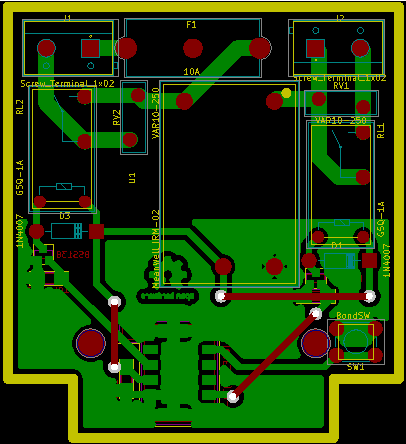
\includegraphics{img/kicad/board.pdf}
\caption{Výkres plošného spoje chytré zásuvky}
\end{figure}

\begin{figure}[H]
\centering
\label{fig:components}
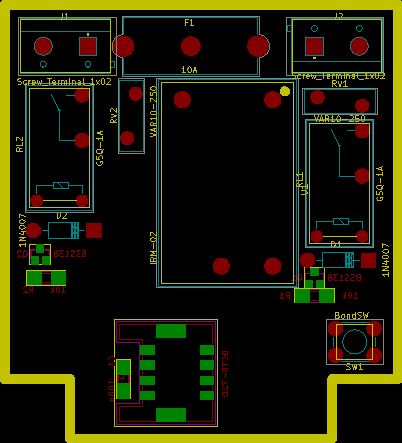
\includegraphics{img/kicad/components.pdf}
\caption{Rozložení součástek na desce plošného spoje chytré zásuvky}
\end{figure}

\newpage

\subsubsection{Rozpiska součástek}

\begin{table}[H]
	\centering
	\begin{tabular}{|l|l|}
		\hline
		\textbf{Značka} & \textbf{Jméno součástky} \\
		\hline
		\hline
		~ & Krabička COMBIPLAST CP-Z-27/B \\
		\hline
		C1 & Keramický SMD 1206 kondenzátor 100~nF \\
		\hline
		D1, D2 & Dioda 1N4007 \\
		\hline
		F1 & Tavná keramická pojistka 10~A 250~VAC \\
		\hline
		IC1 & Bezdrátový modul IQRF DCTR-72DAT \\
		\hline
		~ & Konektoru IQRF KON-SIM-01 pro IC1 \\
		\hline
		J1, J2 & Svorkovnice do DPS\index[zkr]{DPS!Deska plošných spojů|textit} DEGSON DG300-7.5-02P \\
		\hline
		Q1, Q2 & N-MOSFET BSS138 \\
		\hline
		R1, R2 & Rezistor SMD 1206 10~k$\Omega$ \\
		\hline
		RL1, RL2 & Relé OMRON G5Q-1A4-EU 5VDC \\
		\hline
		RV1, RV2 & MOV varistor SR PASSIVES VAR10-250 \\
		\hline
		D3, SW1 & Mikrospínač HIGHLY PB6141FL-13 \\
		\hline
		U1 & Spínaný zdroj MEAN WELL IRM-02-5 \\
		\hline
	\end{tabular}
	\caption{Rozpiska součástek chytré zásuvky}\label{table:rozpiska-soucastek}
\end{table}

\newpage

\subsection{Brána}

Pro bránu jsem použil linuxový jednodeskový počítač Raspberry Pi 2 model B. Bezdrátový modul IQRF DCTR-72DAT je k~bráně připojen přes sběrnici SPI\index[zkr]{SPI!Serial Peripheral Interface|textit} pomocí adaptéru IQRF KON-RASP-01. Pro komunikaci s~GSM sítí lze použít USB\index[zkr]{USB!Universal Serial Bus|textit} GSM\index[zkr]{GSM!Global System for Mobile Communications|textit}\index[zkr]{GSM!Groupe SpécialMobile|textit}/3G modem (například Huawei E3131) nebo starší mobilní telefon (například Samsung Star II nebo Samsung Galaxy Gio). Brána se napájí pomocí externího spínaného zdroje s~microUSB konektorem, který má výstupní napětí 5~V a maximální výstupní proud 2~A.

\begin{figure}[H]
\centering
\label{fig:iqrf/fotka-kon-rasp-01}
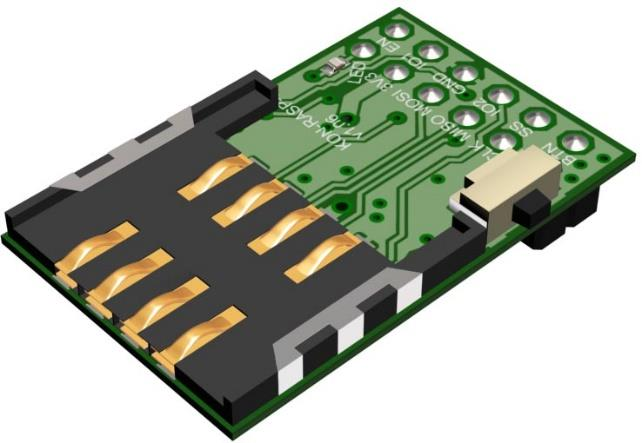
\includegraphics[width = 64mm]{img/iqrf/kon-rasp-01.png}
\caption{Fotografie adaptéru IQRF KON-RASP-01}
\end{figure}

\begin{figure}[H]
\centering
\label{fig:iqrf/zjednodusene-schema-kon-rasp-01}
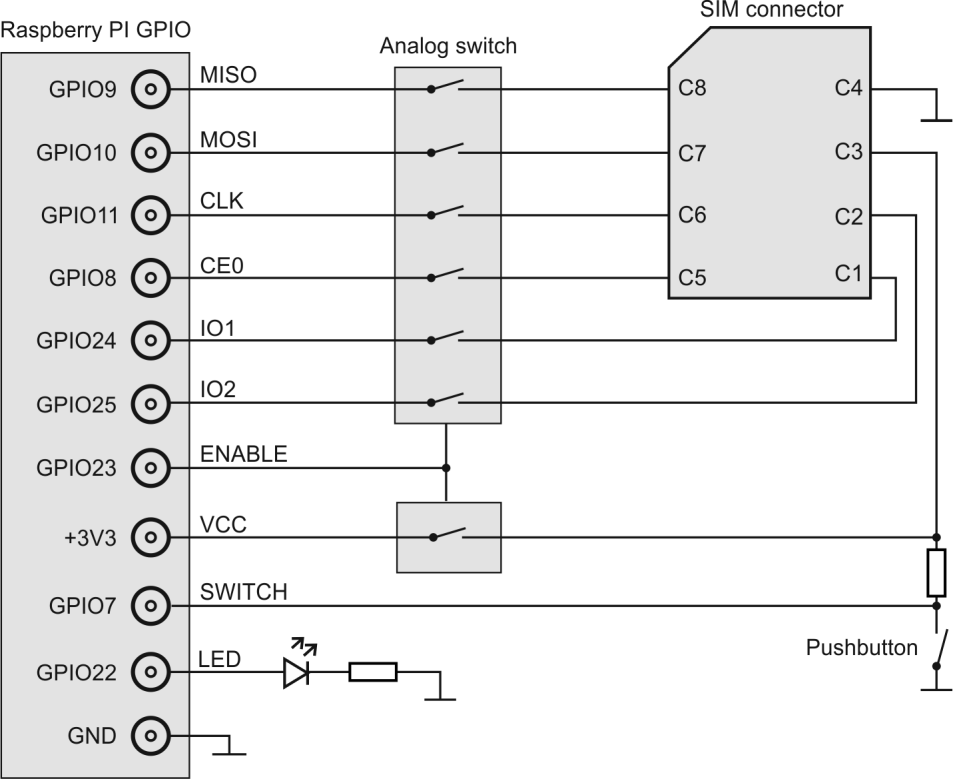
\includegraphics[width = 96mm]{img/iqrf/kon-rasp-01-zjednodusene-schema.png}
\caption{Zjednodušené schéma adaptéru IQRF KON-RASP-01}
\end{figure}

\subsubsection{Raspberry Pi 2 model B}

Raspberry Pi 2 model B je jednodeskový počítač, který má rozměry podobné kreditní kartě. Tento počítač obsahuje:

\begin{itemize}
	\item čtyřjádrový ARM\index[zkr]{ARM!Acorn RISC Machine|textit}\index[zkr]{ARM!Advanced RISC Machine|textit} Cortex-A7 Broadcom BCM2836,
	\item 1~GB operační paměti RAM\index[zkr]{RAM!Random-access memory|textit},
	\item čtyři USB 2.0 porty
	\item port RJ45 pro 100~Mb síťovou kartu,
	\item slot pro microSD\index[zkr]{SD!Secure Digital|textit} kartu,
	\item HDMI\index[zkr]{HDMI!High-Definition Multimedia Interface|textit} výstup,
	\item 40 GPIO\index[zkr]{GPIO!General-purpose input/output|textit} pinů, na kterých jsou vyvedeny sběrnice SPI\index[zkr]{SPI!Serial Peripheral Interface|textit}, I2C\index[zkr]{I2C!Inter-Integrated Circuit|textit}, USART\index[zkr]{USART!Universal Synchronous / Asynchronous Receiver and Transmitter|textit}.
\end{itemize}

\begin{figure}[H]
\centering
\label{fig:foto/rpi2}
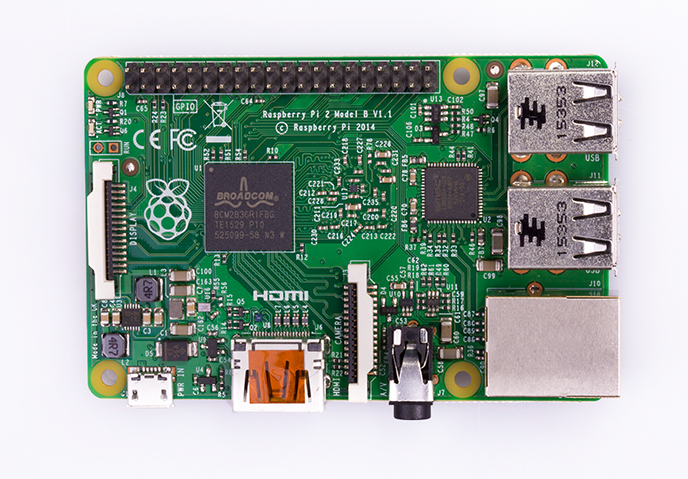
\includegraphics[width = 128mm]{img/foto/rpi2.jpg}
\caption{Fotografie jednodeskového počítače Raspberry Pi 2 model B}
\end{figure}

\newpage

\subsubsection{Blokové schéma brány}

Na obrázku č.~7 se nachází blokové schéma brány, které popisuje její zapojení. Obrázek byl vytvořený v~open-source programu Dia\cite{sw/dia}.

\begin{figure}[H]
\centering
\label{fig:blokove-schema-zasuvky}
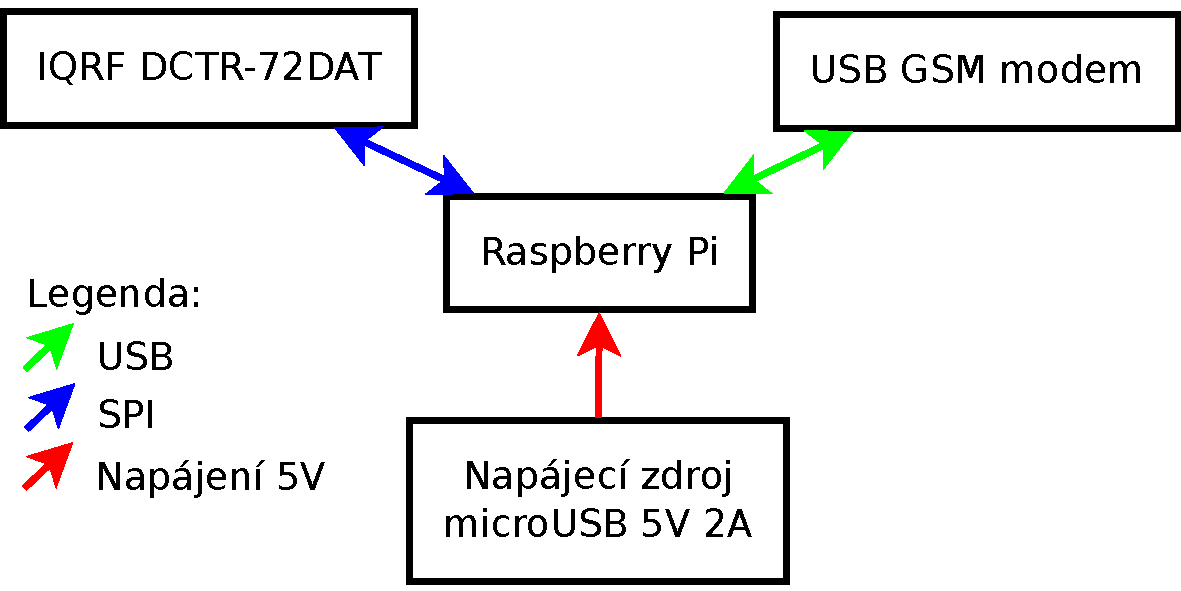
\includegraphics[width = 128mm]{img/blokove-schema/brana.pdf}
\caption{Blokové schéma brány}
\end{figure}

\subsubsection{Rozpiska součástek}

\begin{table}[H]
	\centering
	\begin{tabular}{|l|l|}
		\hline
		%\textbf{Značka} &
    \textbf{Jméno součástky} \\
		\hline
		\hline
		%~ &
    Raspberry Pi 2 model B \\
		\hline
		%~ &
    adaptér IQRF KON-RASP-01 \\
		\hline
		%~ &
    bezdrátový modul IQRF DCTR-72DAT \\
		\hline
		%~ & ~ \\
		%\hline
	\end{tabular}
	\caption{Rozpiska součástek brány}\label{table:rozpiska-soucastek/brana}
\end{table}

\newpage

\section{Návrh software}

\subsection{Komunikace}

Mobilní telefon komunikuje s~bránou pomocí zpráv SMS\index[zkr]{SMS!Short message service|textit}. Brána SMS zprávu zpracuje a pokud je zpráva validní, tak pošle požadavek na chytrou zásuvku přes bezdrátový modul IQRF. Chytrá zásuvka vrátí svůj stav bráně, která poté informuje uživatele, zda byla akce úspěšná.

\begin{figure}[H]
\centering
\label{fig:iqrf/zjednodusene-schema}
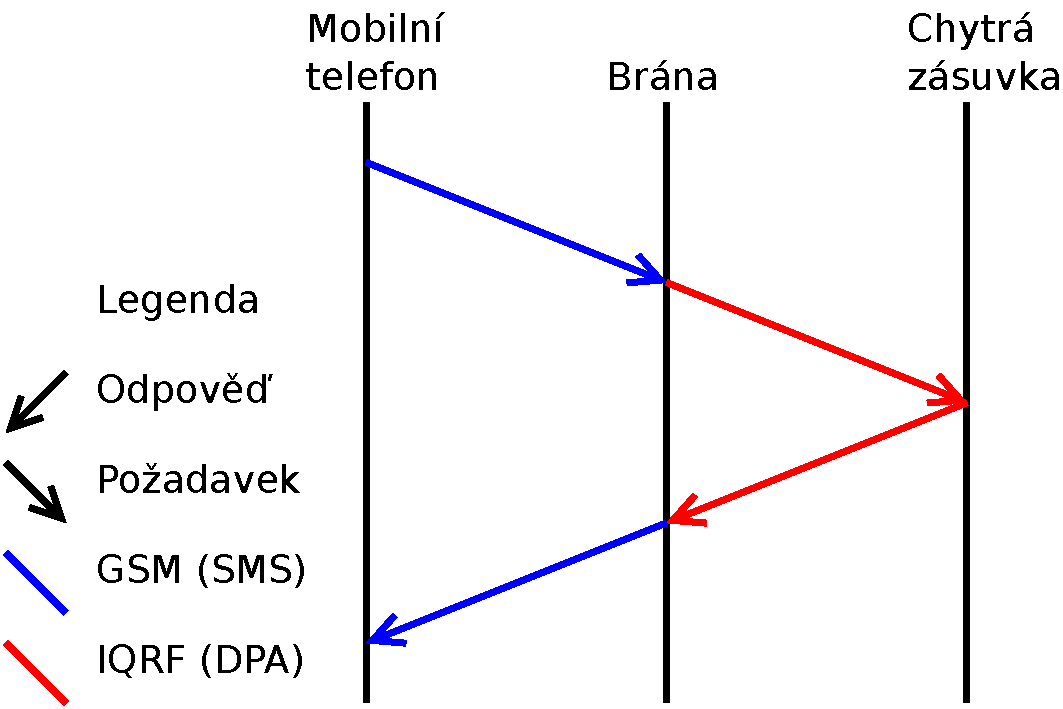
\includegraphics[width = 128mm]{img/blokove-schema/komunikace0.pdf}
\caption{Zjednodušené schéma komunikace}
\end{figure}

\newpage

\subsection{Chytrá zásuvka}

Software chytré zásuvky je psán v~programovacím jazyce C. Software byl napsán ve vývojovém prostředím IQRF IDE\cite{iqrf/ide}\index[zkr]{IDE!Integrated Development Environment|textit}.

\subsubsection{Vývojové prostředí IQRF IDE}

IQRF IDE\cite{iqrf/ide} je zdarma stažitelné vývojové prostředí, které je určené pro vývoj aplikací pro bezdrátové moduly IQRF. Toto vývojové prostředí je pouze pro operační systém Microsoft Windows. Uživatelé operačního systému Apple OS X nebo libovolné linuxové distribuce nemohou vyvíjet software pro tyto bezdrátové moduly. IQRF IDE používá kompilátor CC5X C Compiler\cite{cc5x-compiler}.

\begin{figure}[H]
\centering
\label{fig:iqrf/ide}
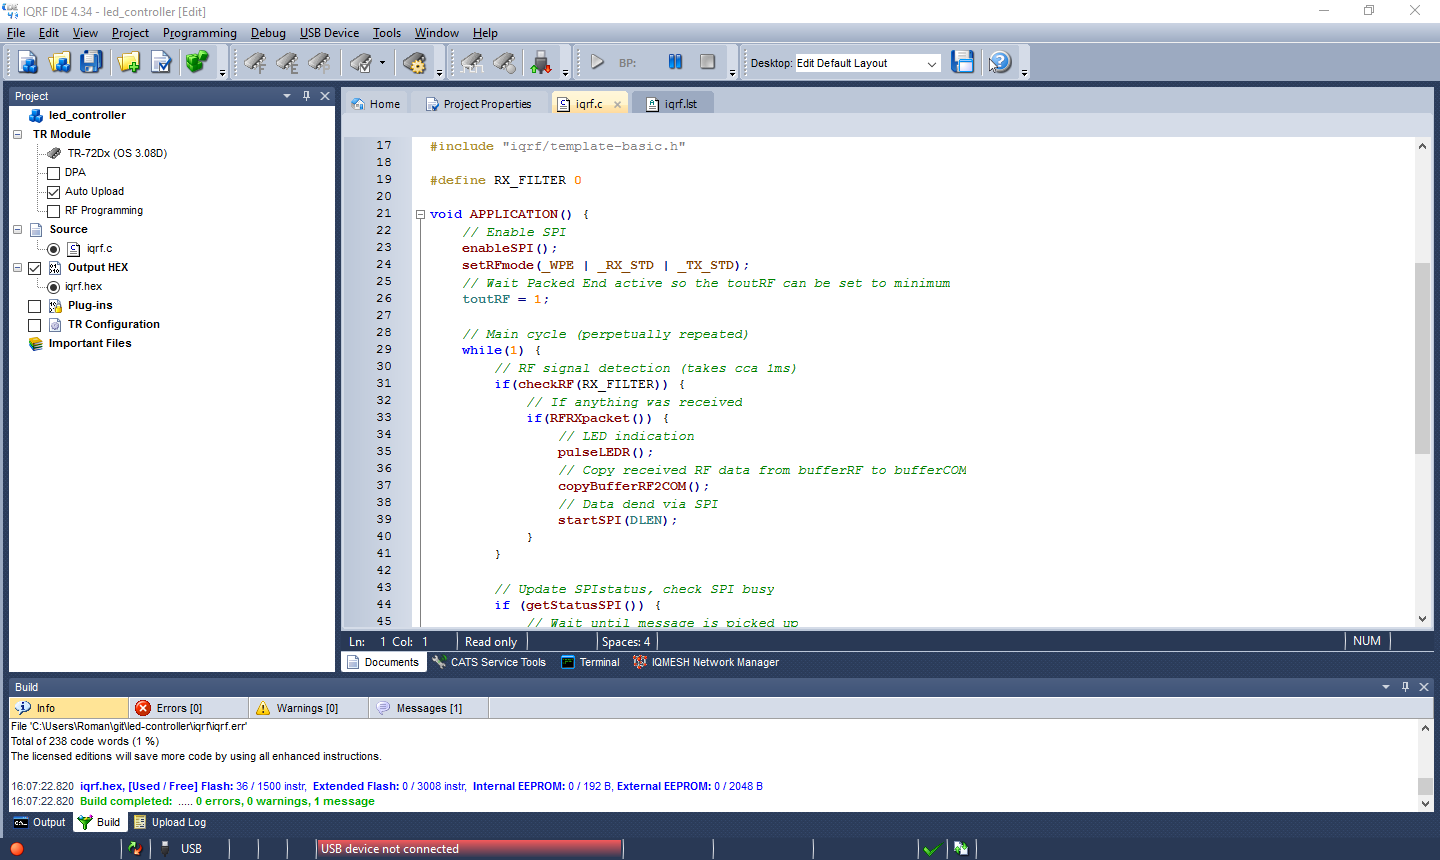
\includegraphics[width = 128mm]{img/iqrf/ide.png}
\caption{Vývojové prostředí IQRF IDE}
\end{figure}

\newpage

\subsubsection{Operační systém IQRF OS}

IQRF OS\cite{iqrf/os} je operační systém určený pro bezdrátové moduly IQRF, pomocí kterého může uživatel jednoduše:

\begin{itemize}
	\item ovládat rádiovou komunikaci,
	\item ovládat komunikaci v~mesh síti,
	\item komunikovat s~periferiemi přes sběrnice SPI, USART, I2C,
	\item pracovat s~pamětmi RAM\index[zkr]{RAM!Random-access memory|textit}, EEPROM\index[zkr]{EEPROM!Electrically Erasable Programmable Read-Only Memory|textit},
	\item inicializovat GPIO,
	\item spínat GPIO,
	\item číst logické hodnoty z~GPIO,
	\item spínat integrované LED\index[zkr]{LED!Light-Emitting Diode|textit} diody,
	\item generovat PWM\index[zkr]{PWM!Pulse Width Modulation|textit} na výstupním pinu,
	\item číst hodnoty z~analogově digitálního převodníku,
	\item číst teplotu z~integrovaného teplotního senzoru.
\end{itemize}

\begin{figure}[H]
\centering
\label{fig:foto/iqrf-os}
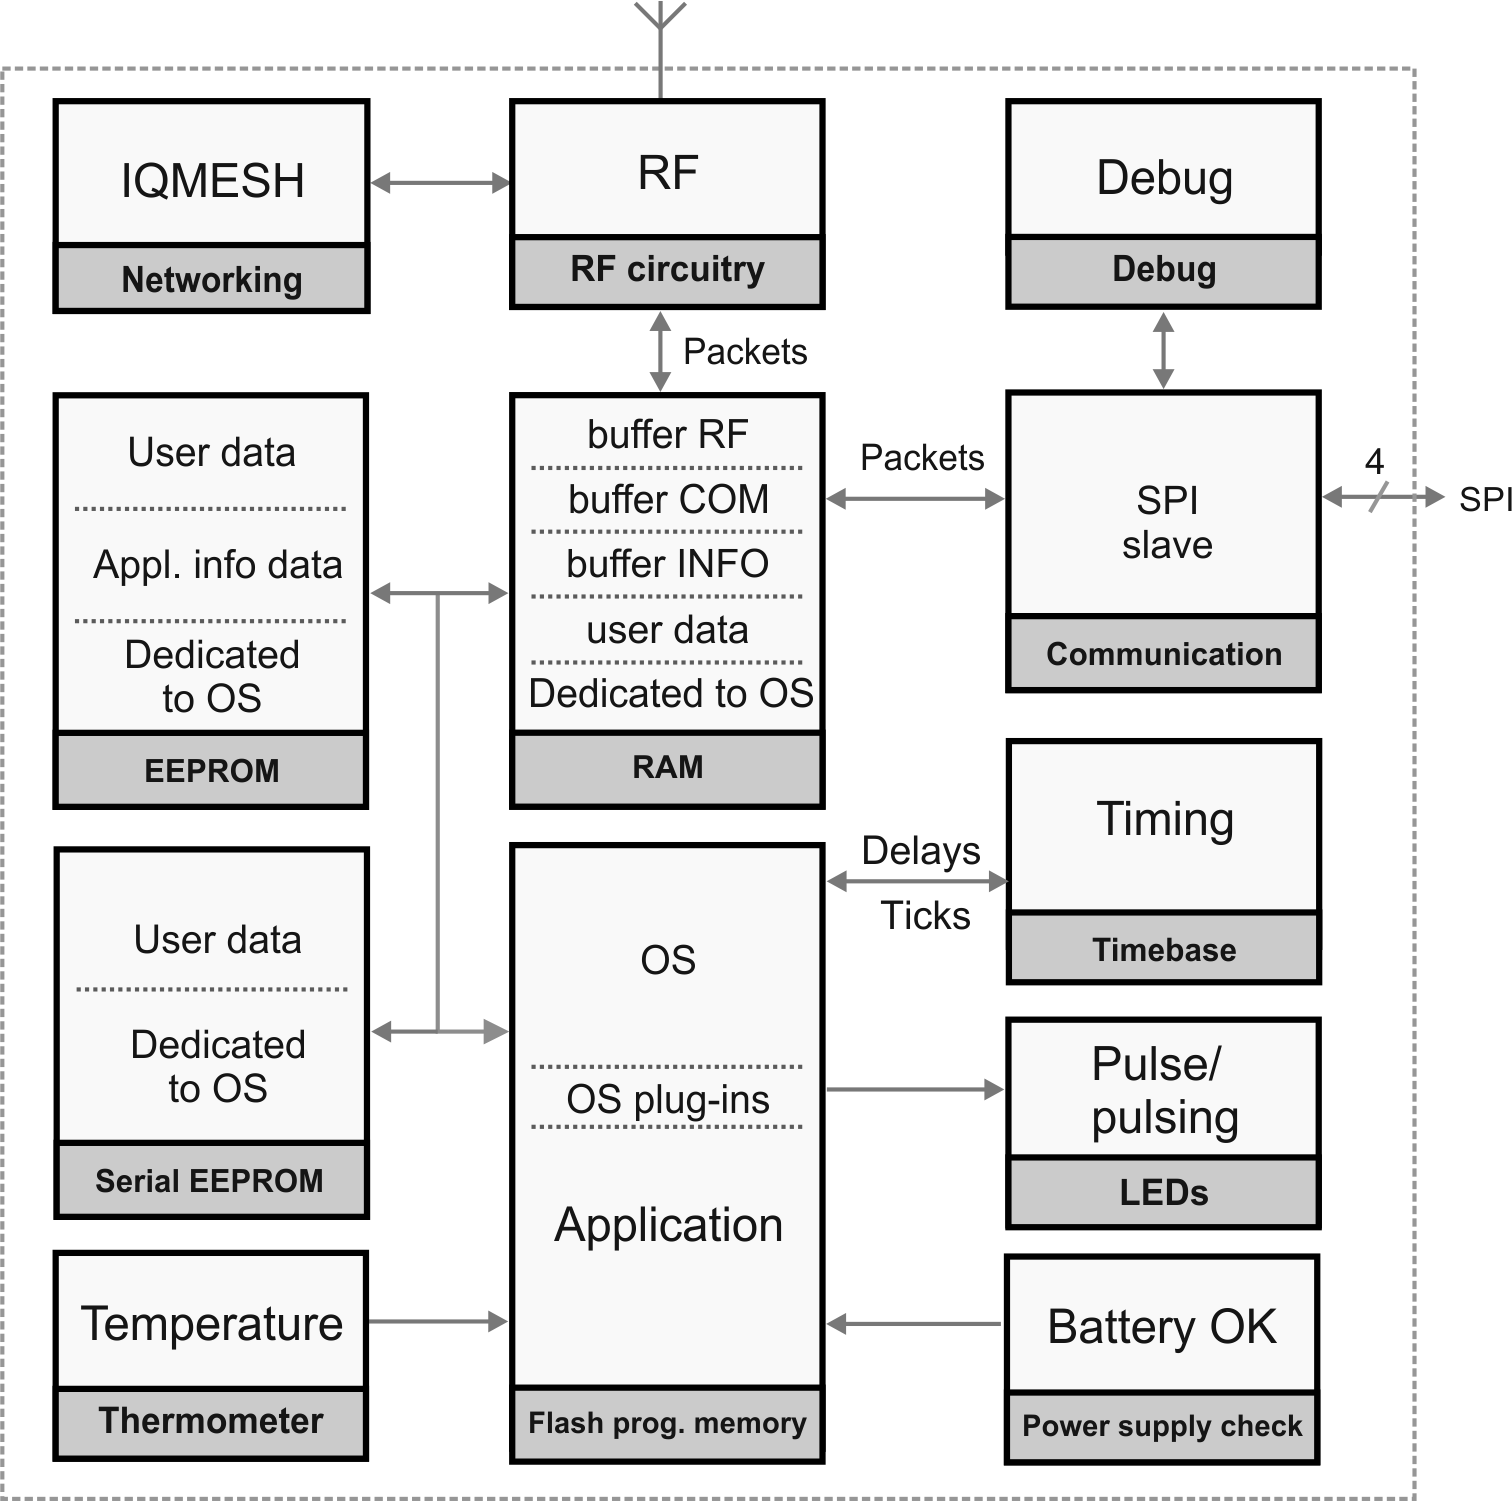
\includegraphics[width = 85mm]{img/iqrf/os-blokove-schema.png}
\caption{Blokové schéma operačního systému IQRF OS}
\end{figure}

\newpage

\subsubsection{Protokol IQRF DPA}

IQRF DPA\cite{iqrf/dpa} je vrstva nad IQRF OS, která se stará o~protokol komunikace IQRF bezdrátových modulů. IQRF DPA má pevně danou strukturu paketů, která je uvedena v~tabulce č.~3. Centrální prvek v~IQRF mesh síti se jmenuje koordinátor, který je umístěn v~bráně. Koordinátor má se své paměti EEPROM uložené informace o~dalších bezdrátových modulech, se kterými má komunikovat. Pokud koordinátor přijme data od bezdrátového modulu, jehož informace nemá uložené v~EEPROM paměti, pak data ignoruje.

\begin{table}[H]
\centering
\begin{tabular}{|c|c|c|c|c|}
\hline
NADR & PNUM & PCMD & HWPID & DATA \\
\hline
siťová adresa & číslo periferie & příkaz & HWP\index[zkr]{HWP!Hardware profile|textit} identifikátor & data \\
\hline
\end{tabular}
\caption{Schéma paketu IQRF DPA}\label{table:iqrf/dpa}
\end{table}

\newpage

\subsection{Brána}

V~bráně běží linuxová distribuce Raspbian, což je speciálně upravená linuxová distribuce pro jednodeskový počítač Raspberry Pi. Tato linuxová distribuce je odvozená od linuxové distribuce Debian, která je jedna z~nejpoužívanějších linuxových distribucích. Software brány je psán v~skriptovacím jazyce Python. Abych si byl jistý, že všechny komponenty softwaru brány fungují, vytvořil jsem pomocí nástroje unittest psal unit testy, které testují důležité komponenty (například čtení konfiguračního souboru). \\

Konfigurační soubor softwaru brány je psán v~datovém formátu YAML\index[zkr]{YAML!YAML Ain't Markup Language|textit}. V~dalším odstavci je uveden ukázkový konfigurační soubor.

\begin{lstlisting}[language=yaml, numbers=left]
gsm:
  enabled: true
  interface: uart
  interfaces:
    uart:
      port: "/dev/ttyUSB0"
      baudRate: 9600
  pin: false

iqrf:
  enabled: true
  interface: spi
  interfaces:
    spi:
      port: "/dev/spidev0.0"
    uart:
      port: "/dev/ttyACM0"
baudRate: 9600
\end{lstlisting}

\newpage

\subsubsection{AT příkazy}

AT příkazy jsou příkazy, které se používají pro komunikaci s~GSM modemem. Dříve se AT příkazům říkalo Hayesovy příkazy (vymyslel je Dennis Hayes pro svůj Hayes Smartmodem 300). Pojmenování AT příkazy vzniklo podle slova \textbf{AT}tention, což v~češtině znamená pozor, upozornit. \\

Základní AT příkaz je příkaz \textit{AT}, který odpoví OK, pokud je vše v~pořádku. Příkaz \textit{ATI} vypisuje informace o~modemu (například výrobce a model). Pomocí příkazu \textit{AT+CMGF=1} lze nastavit textový ASCII\index[zkr]{ASCII!American Standard Code for Information Interchange|textit} přenos dat. \\

Pokud je SIM karta chráněna PIN kódem, pak je možno ji odemknout pomocí příkazu \textit{AT+CPIN=PIN-SIM-KARTY} a poté pomocí příkazu \textit{AT+CPIN?} ověřit, zda byl zadán správný PIN kód. \\

Pomocí příkazu \textit{AT+CMGL=”ALL”} jsou každou sekundu přečteny všechny SMS zprávy, které jsou uloženy na SIM kartě. Odpověď vypadá takto:

\textit{+CMGL: číslo SMS zprávy,"stav zprávy (přečteno/nepřečteno)","telefonní číslo odesílatele",,"datum a čas přijetí SMS zprávy" \\ Text \\ OK}.
Pomocí příkazu \textit{AT+CMGS="telefonní číslo příjemce" \\ Text <26>\footnote{<26> zastupuje ASCII znak Substitute}} se pak odešle SMS zpráva.

Pomocí příkazu \textit{ATD+420123456789;} se \uv{vytočí} telefonní číslo +420123456789. Následně je pomocí příkazu \textit{AT+CHUP} ukončeno spojení.

\begin{table}[H]
	\centering
	\begin{tabular}{|l|l|}
		\hline
		\textbf{Příkaz} & \textbf{Popis} \\
		\hline
		\hline
		AT & Základní AT příkaz \\
		\hline
		ATI & Vypíše informace o~modemu \\
		\hline
		AT+CPIN=1234 & Odemkne SIM kartu pomocí PINu 1234 \\
		\hline
		AT+CPIN? & Odpoví, jestliže je PIN v~pořádku \\
		\hline
		AT+CMGF=1 & Nastavení textového ASCII přenosus dat \\
		\hline
		AT+CMGL=”ALL” & Přečte všechny SMS zprávy \\
		\hline
		AT+CMGS="telefonní číslo příjemce" & Odeslání SMS zprávy \\
		\hline
		ATD+420123456789; & Vytočí číslo +420123456789 \\
		\hline
		AT+CHUP & Zavěšení hovoru (spojení) \\
		\hline
	\end{tabular}
	\caption{Seznam použitých AT příkazů}\label{table:at-prikazy}
\end{table}

\newpage

\section{Technické parametry}

\subsection{Chytrá zásuvka}

\begin{table}[H]
	\centering
	\begin{tabular}{lr}
		\hline
		\textbf{Technické parametry} & ~ \\
		\hline
		\hline
		\textbf{Rozměry} & 7$\times$12$\times$4,5~cm \\
		\textbf{Hmotnost} & x~g \\
		\hline
		\textbf{Elektrické parametry} \\
		\hline
		\hline
		\textbf{Napájecí napětí} & 90~V až 250~V AC\index[zkr]{AC!Alternating current|textit} \\
		\textbf{Maximální odběr proudu} & 400~mA \\
		\textbf{Maximální spínatelný proud} & 10~A \\
		\hline
		\textbf{Ostatní parametry} \\
		\hline
		\hline
		\textbf{Přenos dat} & bezdrátově na frekvenci 868~MHz \\
		\textbf{Protokol} & IQRF DPA \\
	\end{tabular}
	\caption{Parametry chytré zásuvky}\label{table:parametry/chytra-zasuvka}
\end{table}

\subsection{Brána}

\begin{table}[H]
	\centering
	\begin{tabular}{lr}
		\hline
		\textbf{Technické parametry} & ~ \\
		\hline
		\hline
		\textbf{Rozměry} & 7$\times$12$\times$4,5~cm \\
		\textbf{Hmotnost} & x~g \\
		\hline
		\textbf{Elektrické parametry} \\
		\hline
		\hline
		\textbf{Napájecí napětí} & 5~V DC\index[zkr]{DC!Direct current|textit} \\
		\textbf{Maximální odběr proudu} & 2~A \\
	\end{tabular}
	\caption{Parametry brány}\label{table:parametry/zbrana}
\end{table}

\newpage

\section*{Závěr}

\addcontentsline{toc}{section}{Závěr}

Navržený systém dálkového ovládání elektrických spotřebičů byl navržen a realizován ve formě funkčního vzorku. Na obrázcích č.~14 a 15 jsou fotografie funkčního vzorku chytré zásuvky a brány. Funkce chytré zásuvky i celého systému jejího dálkového ovládání pomocí GSM komunikace z~mobilního telefonu vzdáleného uživatele byla ověřena a shledána plně funkční. Výsledkem tohoto projektu je tedy plně funkční chytrá zásuvka, která nejenže splňuje všechny požadavky zadání, ale v~mnoha směrech je i rozšiřuje – například o~zpětný přenos SMS informací vzdálenému uživateli o~okamžitém stavu sepnutí/vypnutí zásuvky. Vzhledem k~charakteru a univerzalitě řešení by systém v~budoucnosti mohl umožnit i zpětný přenos dalších SMS informací (např. teplota v~objektu) nebo ovládání přes Internet.

\begin{figure}[H]
\centering
\label{fig:foto/brana}
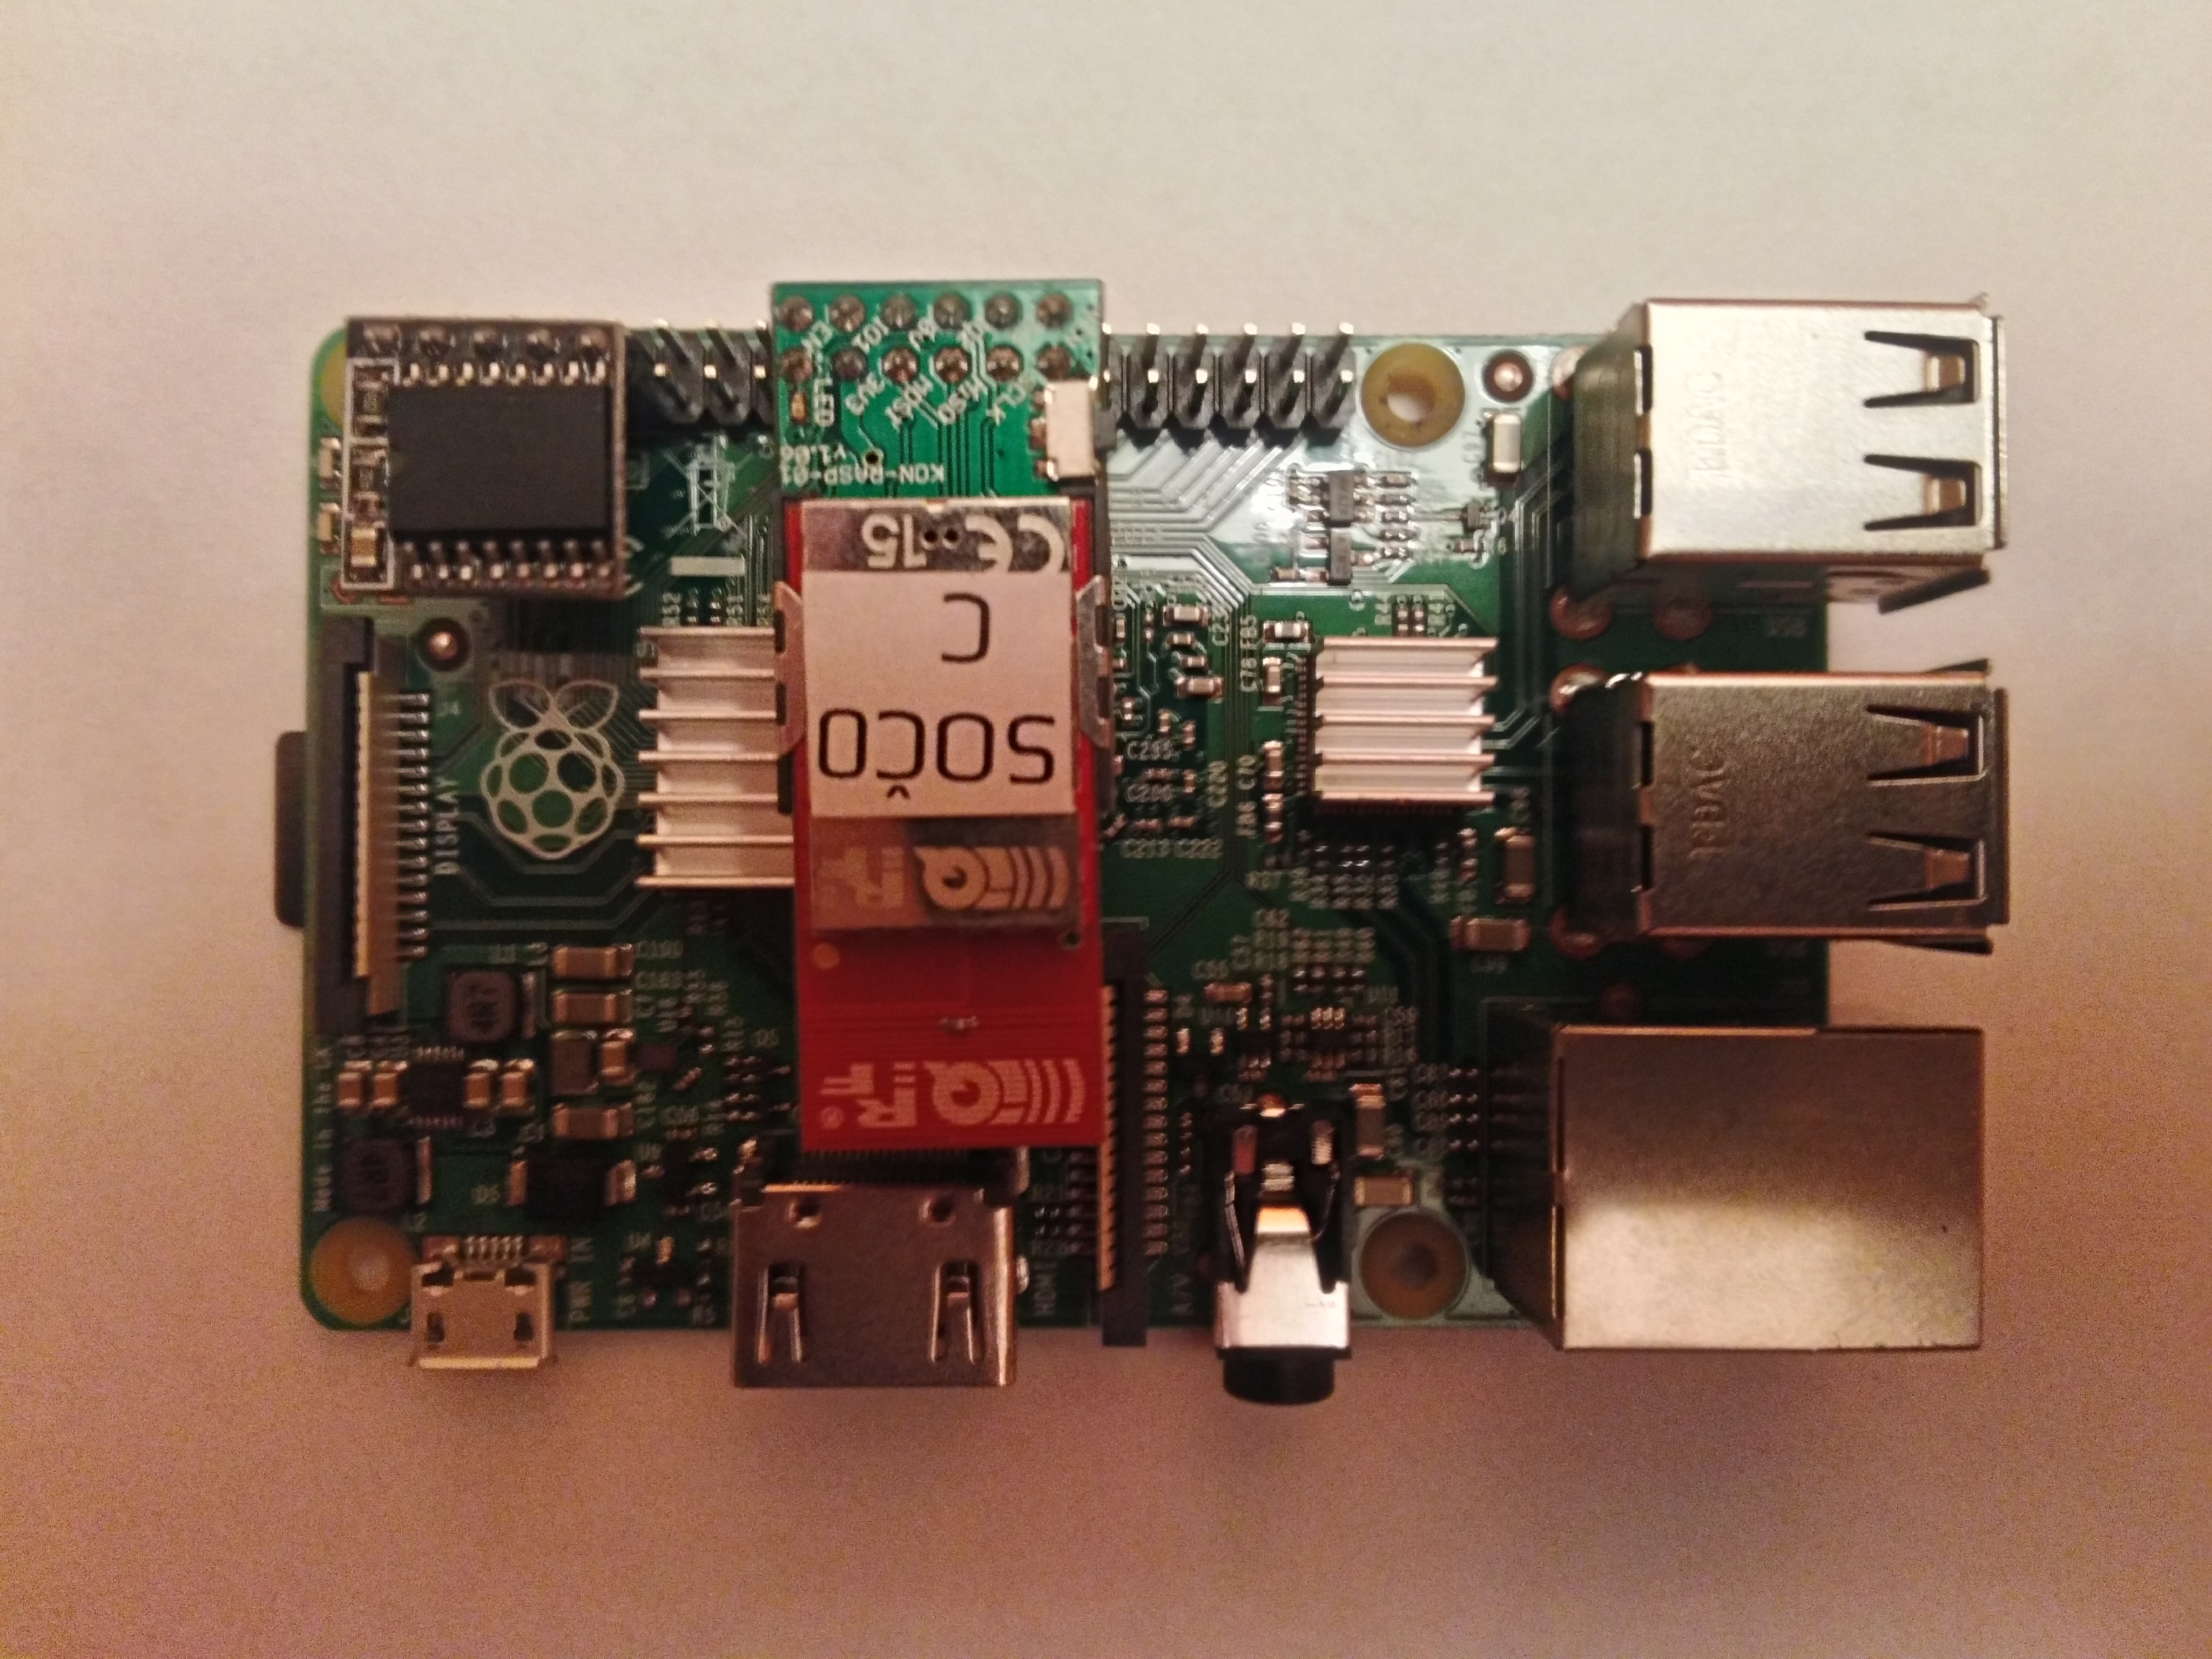
\includegraphics[width = 128mm]{img/foto/brana.jpg}
\caption{Fotografie funkčního vzorku brány}
\end{figure}

\begin{figure}[H]
\centering
\label{fig:foto/brana}
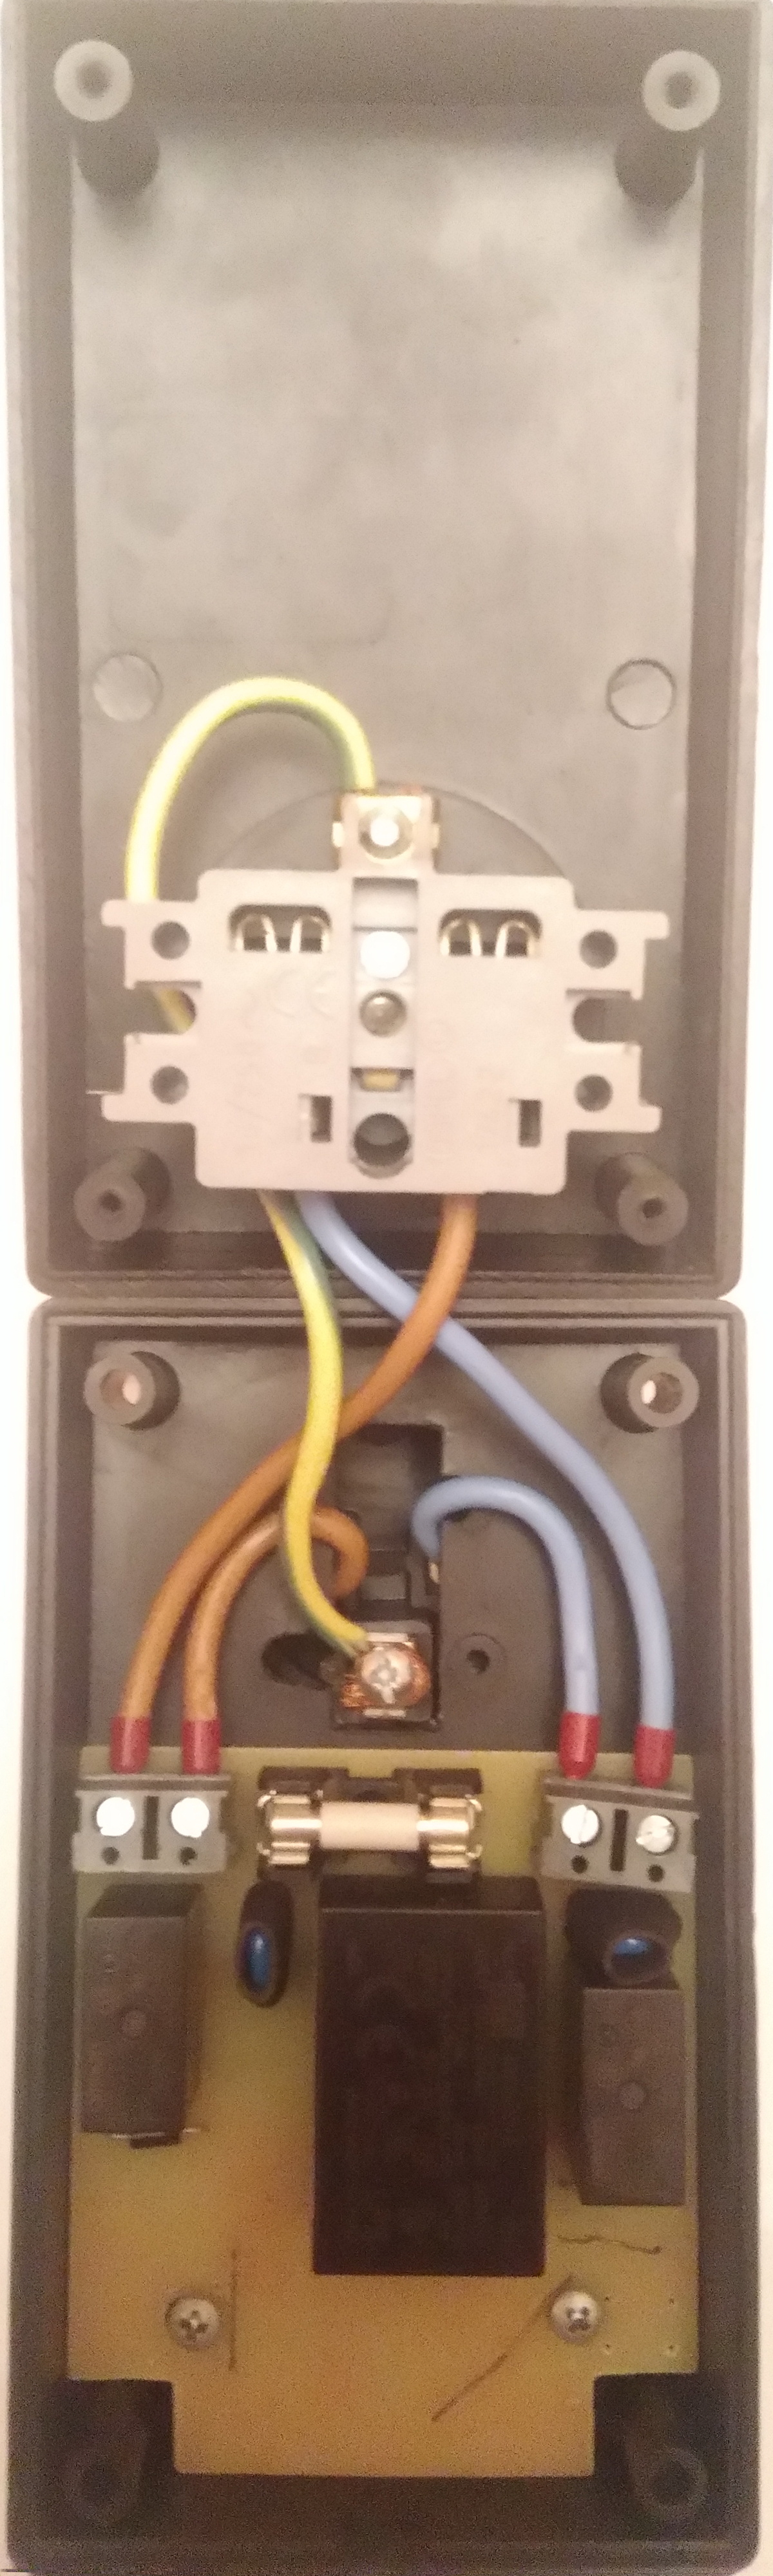
\includegraphics[width = 64mm]{img/foto/zasuvka.jpg}
\caption{Fotografie funkčního vzorku chytré zásuvky}
\end{figure}

\newpage

\printindex[zkr]

\addcontentsline{toc}{section}{Seznam použitých zkratek}

\newpage

\begin{thebibliography}{99}

\addcontentsline{toc}{section}{Seznam použité literatury}

\bibitem{wiki/ism-band}
Wikipedia. ISM\index[zkr]{ISM!Industrial, Scientific and Medical|textit} Band \emph{Wikipedia} [online]. [cit. 2016-01-08]. \\ Dostupné z: \url{https://en.wikipedia.org/wiki/ISM\_band}

\bibitem{wiki/hayes-command-set}
Wikipedia. Hayes command set \emph{Wikipedia} [online]. [cit. 2016-01-08]. \\ Dostupné z: \url{https://en.wikipedia.org/wiki/Hayes\_command\_set}

\bibitem{iqrf/ide}
MICRORISC. IQRF IDE \emph{IQRF} [online]. Jičín, 2016 [cit. 2017-01-09]. \\ Dostupné z: \url{http://iqrf.org/technology/iqrf-ide}

\bibitem{iqrf/os}
MICRORISC. Operating system \emph{IQRF} [online]. Jičín, 2016 [cit. 2017-01-09]. \\ Dostupné z: \url{http://iqrf.org/technology/operating-system}

\bibitem{iqrf/os/guide}
MICRORISC. IQRF OS v3.08D User's guide for TR-7xD \emph{IQRF} [online]. Jičín, 2016 [cit. 2017-01-29]. \\ Dostupné z: \url{http://www.iqrf.org/weben/downloads.php?id=155}

\bibitem{iqrf/dpa}
MICRORISC. DPA \emph{IQRF} [online]. Jičín, 2016 [cit. 2017-01-09]. \\ Dostupné z: \url{http://iqrf.org/technology/dpa}

\bibitem{iqrf/dctr-72d-datasheet}
MICRORISC. Datasheet (DC)TR-72D \emph{IQRF} [online]. Jičín, 2016 [cit. 2017-01-09]. \\ Dostupné z: \url{http://iqrf.org/weben/downloads.php?id=337}

\bibitem{iqrf/kon-rasp-01-datasheet}
MICRORISC. User's guide KON-RASP-01 \emph{IQRF} [online]. Jičín, 2016 [cit. 2017-01-23]. \\ Dostupné z: \url{http://www.iqrf.org/weben/downloads.php?id=412}

\bibitem{microchip/pic16f1938}
MICROCHIP. PIC16F1938 \emph{PIC16F1938} [online]. 2017 [cit. 2017-01-29]. \\ Dostupné z: \url{http://www.microchip.com/wwwproducts/en/PIC16F1938}

\bibitem{robodoupe-mosfet-a-rele}
Jiri Bezstarosti. Tranzistor jako spínač \emph{Robodoupě} [online]. 2012 [cit. 2017-01-09]. \\ Dostupné z: \url{http://robodoupe.cz/2012/tranzistor-jako-spinac/}

\bibitem{faze-vlevo-nebo-vpravo}
Jaroslav Borovec. Fáze vlevo nebo vpravo, v~čem tkví nebezpečí? \emph{Eletrika.cz} [online]. 2009 [cit. 2017-01-09]. \\ Dostupné z: \url{http://elektrika.cz/clanky/faze-vlevo-nebo-vpravo-v-cem-tkvi-nebezpeci}

\bibitem{zasuvka-typ-e}
Oldřich Mrázek. Přehled zásuvek používaných ve světě - Typ E \emph{HW Server} [online]. 2009 [cit. 2017-01-09]. \\ Dostupné z: \url{http://zasuvky.hw.cz/index2.php#E}

\bibitem{teardown-wemo-switch}
Brian Dipert. Teardown: WeMo Switch is highly integrated \emph{EDN} [online]. 2015 [cit. 2017-01-09]. \\ Dostupné z: \url{http://www.edn.com/design/consumer/4440797/Teardown--WeMo-Switch-is-highly-integrated}

\bibitem{sw/dia}
Dia \emph{Dia} [online]. [cit. 2017-01-19]. \\ Dostupné z: \url{https://wiki.gnome.org/Apps/Dia/}

\bibitem{sw/kicad}
KiCad EDA\index[zkr]{EDA!Electronic design automation|textit} \emph{KiCad EDA} [online]. [cit. 2017-01-19]. \\ Dostupné z: \url{http://kicad-pcb.org/}

\bibitem{cc5x-compiler}
B Knudsen Data. CC5X C Compiler \emph{CC5X} [online]. Norsko, 2016 [cit. 2017-01-29]. \\ Dostupné z: \url{http://www.bknd.com/cc5x/}

\end{thebibliography}

\newpage

\listoffigures

\addcontentsline{toc}{section}{Seznam obrázků}

\listoftables

\addcontentsline{toc}{section}{Seznam tabulek}

\end{document}
